\subsection{Caricamento di una Rete Bayesiana}\label{ReteB}

L'Operazione di caricamento della rete Bayesiana consta di due passaggi fondamentali:
\begin{enumerate}
	\item \textbf{Passaggio 1} L'utente accede al pannello di selezione della rete bayesiana cliccando il pulsante \textbf{Upload .json file} presente in Figura \ref{Pannello};
	\item \textbf{Passaggio 2} L'utente seleziona, tra i files presenti nella propria macchina, la rete bayesiana che desidera caricare e preme il pulsante \textbf{Apri} (Figura \ref{UploadRete}).
\end{enumerate} 

\begin{figure}[H]
	\begin{center}
		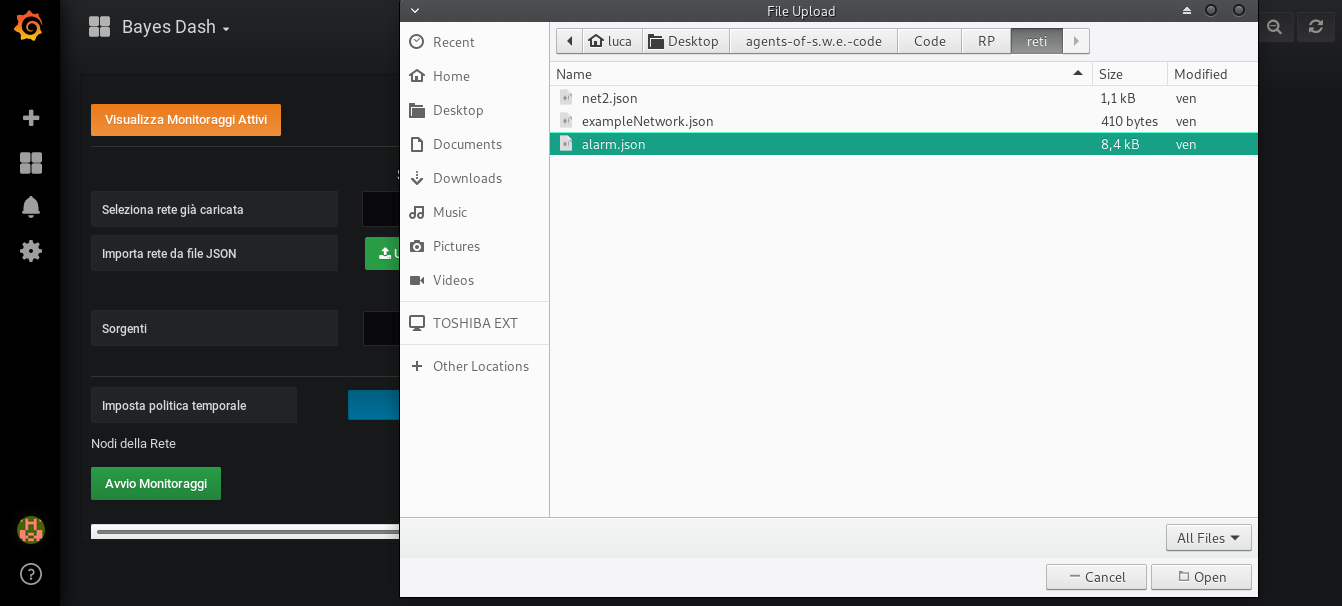
\includegraphics[scale=0.3]{./images/UpRete.png}
		 \caption{Pannello di caricamento Rete Bayesiana}	
		 \label{UploadRete}
	\end{center}
\end{figure}

L'estensione accettata dal plug-in per il file di definizione della rete è \textit{.json}. La rete bayesiana deve essere ben formata, seguendo le direttive della libreria \textit{JSBayes}. Inoltre la rete deve contenere un identificativo del proprio nominativo, necessario al momento del salvataggio della rete nel server.\\
~\\
Al seguito del corretto caricamento della rete bayesiana l'utente verrà avvisato del buon esito dell'operazione da un messaggio di notifica. Verrà inoltre visualizzato nel pannello \textit{G\&B} la lista dei nodi di cui è composta la rete bayesiana caricata (Figura \ref{NodiRete}).

\begin{figure}[H]
	\begin{center}
		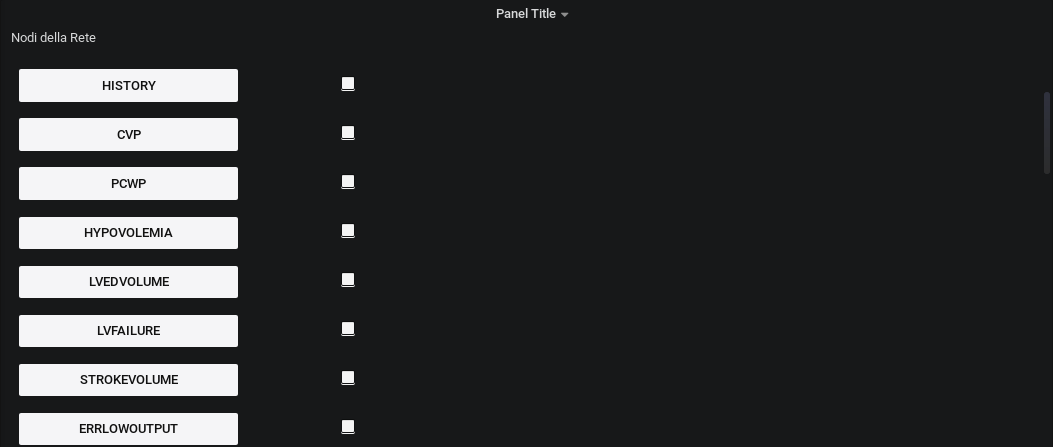
\includegraphics[scale=0.35]{./images/NodiRete.png}
		 \caption{Visualizzazione dei nodi della rete bayesiana caricata}	
		 \label{NodiRete}
	\end{center}
\end{figure}

Nel caso l'utente stesse visualizzando una diversa rete bayesiana prima del caricamento del nuovo file questa viene memorizzata nel server insieme alle sue eventuali impostazioni di collegamento.

~\\
\textbf{\textcolor{red}{ATTENZIONE}}: Nel caso in cui l'utente abbia selezionato per il caricamento un file di definizione della rete non conforme alle direttive della libreria \textit{JSBayes}, l'operazione non andrà a buon fine e l'utente verrà avvisato attraverso un apposito messagio d'errore (Figura \ref{ErroreUpRete}).

\begin{figure}[H]
	\begin{center}
		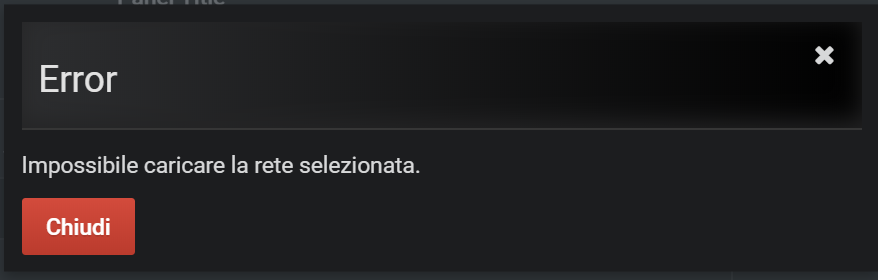
\includegraphics[scale=0.6]{./images/ErroreUpRete.png}
		 \caption{Messaggio di Errore caricamento Rete Bayesiana}	
		 \label{ErroreUpRete}
	\end{center}
\end{figure}

